\subsection{调度延迟敏感性与软件费用事后复核}
\label{sec:ch5-delay-audit}

为连接路径质量与调度费用，补充学习配额、强配额随机和贪心修复三个方法的原确认轨迹复核。每方法仍为十训练块、五工作负载、每负载六回合与每回合1000步，即每方法300回合，三方法共900回合。重放读取原卸载动作，由冻结上层重现位置决策；在请求刷新前采集实际路径时延与截止时间。逐步指标、请求计数、外生流、检查点和模型摘要均与原记录核对。该过程未训练或筛选模型，也未把新延迟回写状态。

第一类评分对所有方法施加共同附加等待 $\delta\in\{0,20,50,100,150\}\,\mathrm{ms}$，把原成功条件替换为 $T_m+\delta\leq D_m$，未接纳请求仍计入原生成分母。第二类评分按训练块、负载、回合和步号配对原隔离计时记录，使用该方法每次完整软件调用时间 $c_t$ 判断 $T_m+c_t\leq D_m$；不以平均或p95时间替代逐次费用。两类均先汇总块内成功与生成计数，再计算十块等权均值和逐项配对 $t$ 区间。它们是原轨迹上的探索性事后评分，不扩充独立训练重复数，也不改变预定主检验族。

\begin{table}[!htbp]
 \centering
 \bicaption{附加延迟及逐次软件费用事后评分（DSR为百分比，差值及区间为百分点）}{Post-hoc scoring with added delay and per-call software costs}
 \label{tab:ch5-delay-audit}
 \footnotesize
 \setlength{\tabcolsep}{3pt}
 \begin{tabular}{lrrrll}
  \toprule
  评分条件 & 学习 & 强随机 & 贪心 & 学习减强随机（95\%区间） & 学习减贪心（95\%区间） \\
  \midrule
  0 ms & 34.244 & 34.100 & 32.821 & $+0.143\ [0.006,0.281]$ & $+1.423\ [1.258,1.587]$ \\
  20 ms & 32.700 & 32.581 & 31.803 & $+0.119\ [-0.013,0.251]$ & $+0.897\ [0.748,1.046]$ \\
  50 ms & 30.603 & 30.506 & 30.294 & $+0.097\ [-0.029,0.223]$ & $+0.309\ [0.159,0.459]$ \\
  100 ms & 27.871 & 27.746 & 28.199 & $+0.125\ [0.017,0.232]$ & $-0.329\ [-0.498,-0.160]$ \\
  150 ms & 25.860 & 25.670 & 26.587 & $+0.190\ [0.082,0.298]$ & $-0.728\ [-0.916,-0.540]$ \\
  逐次软件费用 & 29.379 & 30.073 & 32.161 & $-0.694\ [-1.272,-0.116]$ & $-2.782\ [-3.374,-2.190]$ \\
  \bottomrule
 \end{tabular}
\end{table}

\begin{figure}[!htbp]
 \centering
 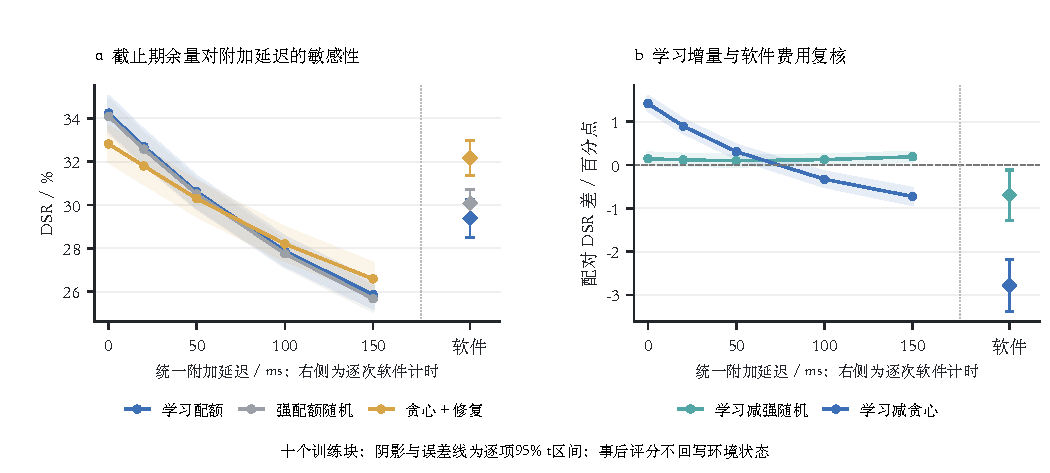
\includegraphics[width=0.98\textwidth]{../docs/figures/图5-20_调度延迟敏感性}
 \bicaption{原确认轨迹的调度延迟敏感性。左面板为DSR，右面板为学习相对强随机和贪心的配对差；菱形单独表示逐次软件费用评分，与共同延迟曲线分开。阴影与误差线为十块逐项95\% t区间，状态不回写}{Scheduling-delay sensitivity on original confirmation trajectories; diamonds denote per-call software scoring, with pointwise ten-block t intervals and no state write-back}
 \label{fig:ch5-delay-audit}
\end{figure}

零附加延迟精确复现原三方法DSR。共同等待增大后，各方法DSR下降，但差值并非固定平移：100 ms时学习减贪心为 $-0.329$ 个百分点，150 ms时为 $-0.728$，说明原学习分配的截止期余量对等待更敏感。学习对强随机的差仍较小，20和50 ms逐项区间跨零；该探索性分析不构成独立确认。

逐次软件费用评分下，学习、强随机和贪心的DSR分别为 $29.379\%$、$30.073\%$ 和 $32.161\%$。学习减强随机为 $-0.694$ 个百分点，逐项区间 $[-1.272,-0.116]$；学习减贪心为 $-2.782$，区间 $[-3.374,-2.190]$。原批次质量优势在这一费用口径下发生反转。因此，指定服务器上的软件调用门槛与计入求解等待后的服务优势须分别判断，预算受限时应把较低的软件费用纳入方法选择。

已接纳请求中，路径时延超过一秒的比例在学习、强随机和贪心中分别约为 $64.06\%$、$64.77\%$ 和 $62.52\%$，进一步说明决策步长与解析完成时间并不等价。上述评分保留原动作、缓存、电量和位置轨迹，没有模拟等待引起的资源占用或后续状态改变；它能够界定原请求的截止期余量，但不是通信受限或持续排队环境的新闭环结果。

